\documentclass[letterpaper,11pt]{memoir}
  \usepackage[utf8]{inputenc}
  \usepackage{fourier}                 % texte en Utopia
  \usepackage[scaled=0.82]{beramono}   % code en Bera
  \renewcommand{\sfdefault}{Myriad-LF} % titres en MyriadPro
  \usepackage{natbib,url}
  \usepackage[english,francais]{babel}
  \usepackage[autolanguage]{numprint}
  \usepackage{vgmath,actu,amsmath,amsthm,amsthm,amsfonts,icomma}
  \usepackage[noae]{Sweave}
  \usepackage[alwaysadjust]{paralist}
  \usepackage{textpos}
  \usepackage{graphicx,color}
  \usepackage{MnSymbol,applekeys}      % symboles spéciaux
  \usepackage{expdlist}
  \usepackage{listingsutf8,answers}
  \usepackage{pdfpages}                % couvertures

  %%%  Couleurs
  \definecolor{comments}{rgb}{0.7,0,0}
  \definecolor{darkred}{rgb}{0.8,0,0}
  \definecolor{shadecolor}{gray}{0}
  \definecolor{link}{rgb}{0,0,0.3}

  %%% Hyperliens
  \usepackage{hyperref}
  \hypersetup{colorlinks,allcolors=link}

  %%% ============
  %%%  Page titre
  %%% ============
  \title{\HUGE
    \fontseries{b}\selectfont ACT 2002 \\
    \fontseries{b}\selectfont Méthodes numériques \\
    \fontseries{m}\selectfont en \\
    \fontseries{b}\selectfont actuariat \\[10mm]
    \huge
    \fontseries{m}\selectfont Partie II \\
    \fontseries{m}\selectfont Simulation stochastique}
  \author{\Large Vincent Goulet \\[3mm]
    \large École d'actuariat, Université Laval}
  \date{\large Notes de cours et exercices}

  %%% ===================
  %%%  STYLE DU DOCUMENT
  %%% ===================

  %% Titres des chapitres
  \chapterstyle{hangnum}
  \renewcommand{\chaptitlefont}{\normalfont\Huge\sffamily\bfseries\raggedright}

  %% Marges, entêtes et pieds de page
  \setlength{\marginparsep}{7mm}
  \setlength{\marginparwidth}{13mm}
  \setlength{\headwidth}{\textwidth}
  \addtolength{\headwidth}{\marginparsep}
  \addtolength{\headwidth}{\marginparwidth}

  %% Titres des sections et sous-sections
  \setsecheadstyle{\normalfont\Large\sffamily\bfseries\raggedright}
  \setsubsecheadstyle{\normalfont\large\sffamily\bfseries\raggedright}
  \maxsecnumdepth{subsection}
  \setsecnumdepth{subsection}

  %% Franciser le second niveau des énumérations
  \setdefaultenum{}{a)}{}{}

  %% Noms de fonctions, code, etc.
  \newcommand{\code}[1]{\texttt{#1}}

  %% Environnements d'exemples et al.
  \theoremstyle{plain}
  \newtheorem{algorithme}{Algorithme}[chapter]
  \newtheorem{thm}{Théorème}[chapter]

  \theoremstyle{definition}
  \newtheorem{exemple}{Exemple}[chapter]
  \newtheorem{definition}{Définition}[chapter]
  \newtheorem*{astuce}{Astuce}

  \theoremstyle{remark}
  \newtheorem*{remarque}{Remarque}
  \newtheorem*{remarques}{Remarques}
  \newenvironment{rem}{\begin{remarque} \mbox{}}{\end{remarque}}
  \newenvironment{rems}{\begin{remarques} \mbox{}}{\end{remarques}}

  %% Options de babel
  \frenchbsetup{CompactItemize=false,%
    ThinSpaceInFrenchNumbers=true,
    ItemLabeli=$\filledtriangleright$,
    ItemLabelii=\textendash}
  \addto\captionsfrench{\def\figurename{{\scshape Fig.}}}
  \addto\captionsfrench{\def\tablename{{\scshape Tab.}}}

  %%% =========================
  %%%  Nouveaux environnements
  %%% =========================

  %% Listes d'objectifs au début des chapitres
  \newenvironment{objectifs}{%
    \noindent
    \begin{framed}
      \vspace{-1.33\baselineskip}
      \begin{shaded}
        \noindent\sffamily\bfseries\textcolor{white}{Objectifs du chapitre}
      \end{shaded}
      \vspace{-0.6\baselineskip}
      \begin{compactitem}
        \small}
      {\end{compactitem}
    \end{framed}}

  %% Environnements de Sweave
  \DefineVerbatimEnvironment{Sinput}{Verbatim}{xleftmargin=\parindent}
  \DefineVerbatimEnvironment{Soutput}{Verbatim}{xleftmargin=\parindent}
  \DefineVerbatimEnvironment{Scode}{Verbatim}{xleftmargin=\parindent}
  \fvset{listparameters={\setlength{\topsep}{0pt}}}
  \renewenvironment{Schunk}{\vspace{\topsep}}{\vspace{\topsep}}

  %% Exercices et réponses
  \Newassociation{sol}{solution}{solutions}
  \Newassociation{rep}{reponse}{reponses}
  \newcounter{exercice}[chapter]
  \newenvironment{exercice}{%
    \begin{list}{\bfseries \thechapter.\arabic{exercice}}{%
        \refstepcounter{exercice}
        \settowidth{\labelwidth}{\bfseries \thechapter.\arabic{exercice}}
        \setlength{\leftmargin}{\labelwidth}
        \addtolength{\leftmargin}{\labelsep}
        \setdefaultenum{a)}{i)}{}{}}\item}
    {\end{list}}
  \renewenvironment{reponse}[1]{%
    \begin{list}{\bfseries #1}{%
        \settowidth{\labelwidth}{#1}
        \setlength{\leftmargin}{\labelwidth}
        \addtolength{\leftmargin}{\labelsep}
        \setdefaultenum{a)}{i)}{}{}}\item}
    {\end{list}}
  \renewcommand{\reponseparams}{{\thechapter.\theexercice}}
  \renewenvironment{solution}[1]{%
    \begin{list}{\bfseries #1}{%
        \settowidth{\labelwidth}{#1}
        \setlength{\leftmargin}{\labelwidth}
        \addtolength{\leftmargin}{\labelsep}
        \setdefaultenum{a)}{i)}{}{}}\item}
    {\end{list}}
  \renewcommand{\solutionparams}{{\thechapter.\theexercice}}

  %%% Remarques importantes
  \newenvironment{gotoR}{%
    \begin{framed}%
      \noindent
      \begin{minipage}{0.07\linewidth}
        \raisebox{-0.5em}[0em][0em]{\LARGE\color{darkred}\noway}
      \end{minipage}
      \begin{minipage}[t]{0.88\linewidth}}
      {\end{minipage}%
    \end{framed}}

  %%% =============================================
  %%%  Paramètres pour les sections de code source
  %%% =============================================
  \lstloadlanguages{R}
  \lstset{language=R,
    extendedchars=true,
    inputencoding=utf8/latin1,
    basicstyle=\small\ttfamily,
    commentstyle=\color{comments}\slshape,
    keywordstyle=\mdseries,
    showstringspaces=false}

  %%% =====================
  %%%  Nouvelles commandes
  %%% =====================
  \newcommand{\R}{\marginpar[\hfill \sffamily R]{\sffamily R}}
  \newcommand{\Splus}{\marginpar[\hfill S$+$]{S$+$}}
  \newcommand{\warning}{\marginpar{\LARGE\danger}}
  \newcommand{\ieee}[3]{\fbox{#1}\hspace{2pt}\fbox{#2}\hspace{2pt}\fbox{#3}}
  \newcommand{\fl}{\mathrm{fl}}
  \newcommand{\tr}{\mathrm{tr}}

  %%% Sous-tableaux et sous-figures
  \newsubfloat{table}
  \newsubfloat{figure}

  %%% Style de la bibliographie
  \bibliographystyle{francais}

  %%% Numérotation des chapitres
  \setcounter{chapter}{6}

%  \includeonly{arithmetique_ordinateurs}

\begin{document}

\frontmatter

\pagestyle{empty}
%%%% Page couverture avant. Il faut modifier la largeur des graphiques
%%% puisque Sweave la règle à 0.8\textwidth.
\setkeys{Gin}{width=\paperwidth}
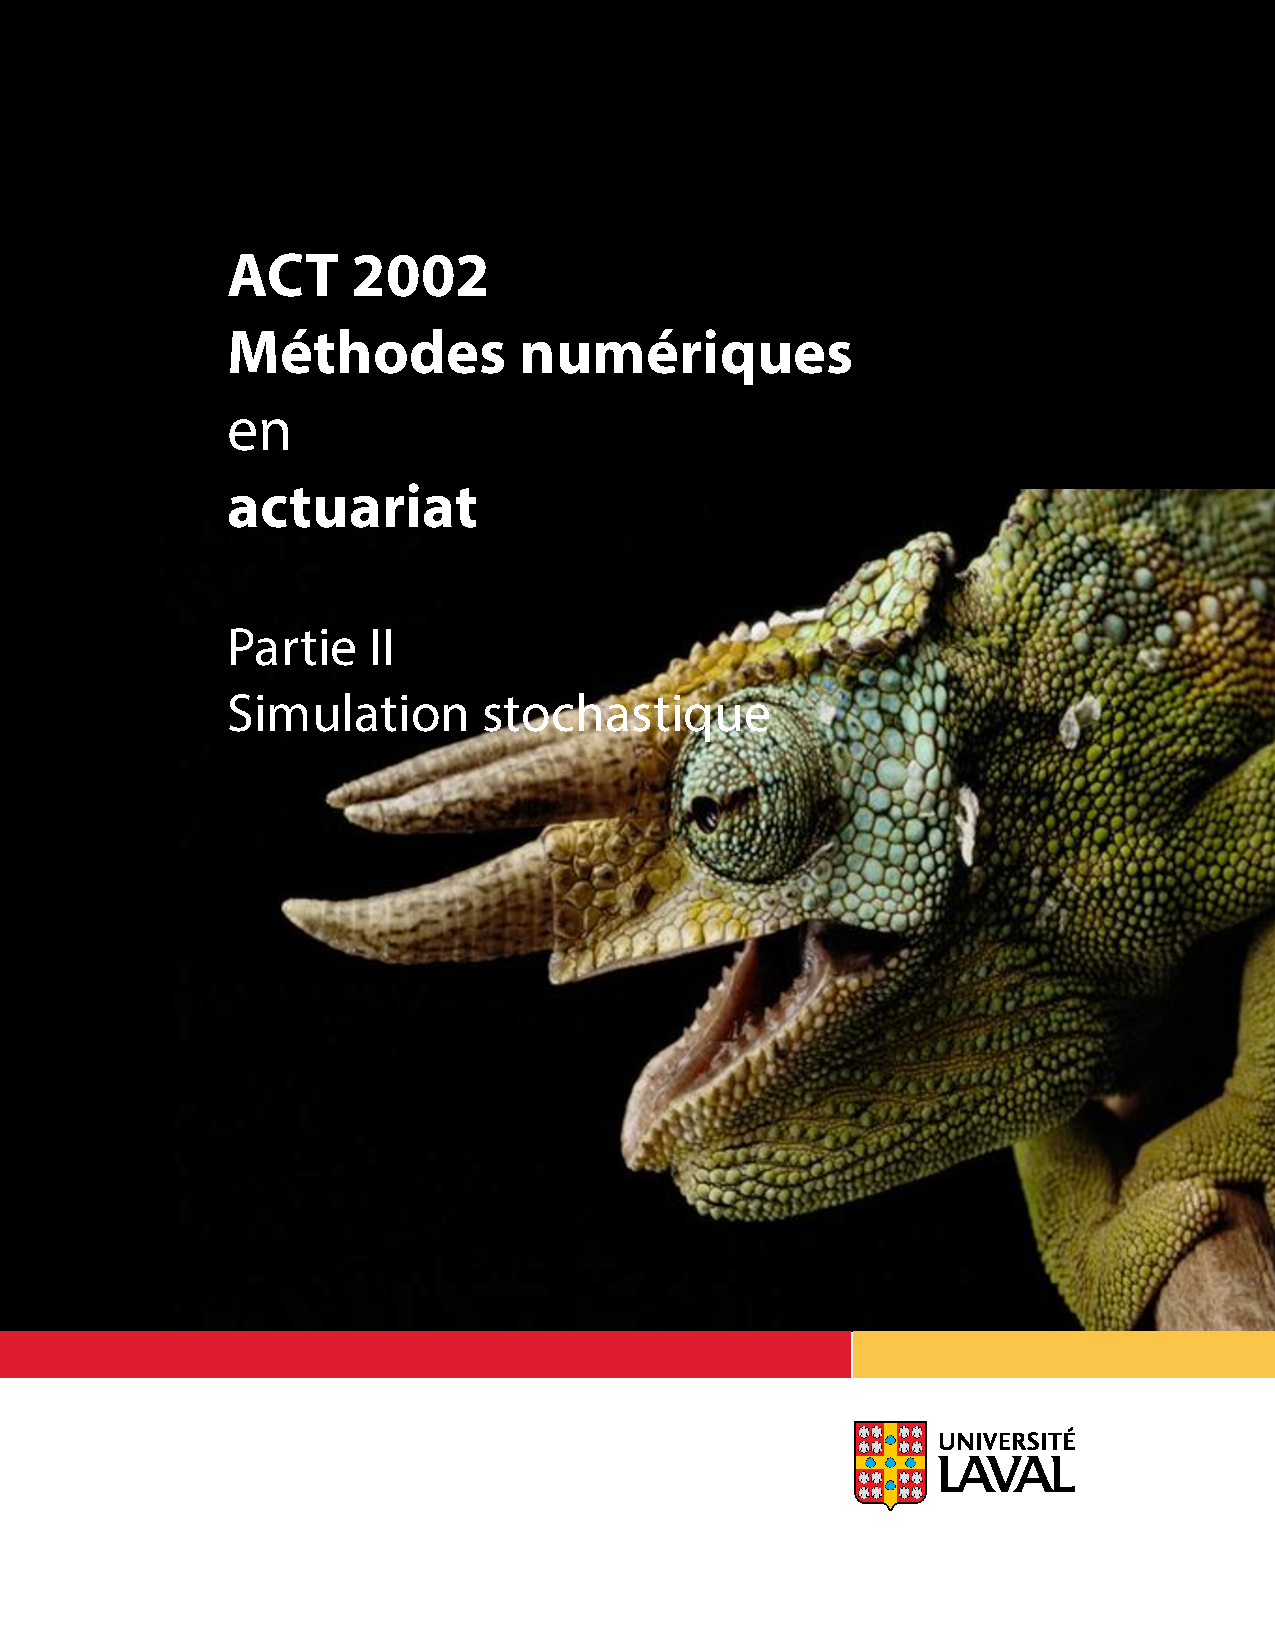
\includepdf[pages=1]{couvertures-partie_2}
\setkeys{Gin}{width=0.8\textwidth}

\cleardoublepage

%%% Page de garde
\begin{adjustwidth*}{13.1mm}{-72mm}
  \sffamily
  \raggedright
  \vspace*{5mm}
  \thetitle \\
  \vspace*{3cm}
  \theauthor \\
  \vspace*{\fill}
  \thedate
\end{adjustwidth*}
\clearpage

%%% Page de notices
\begingroup
\calccentering{\unitlength}
\begin{adjustwidth*}{\unitlength}{-\unitlength}
  \small
  \setlength{\parindent}{0pt}
  \setlength{\parskip}{\baselineskip}

  {\textcopyright} 2012 Vincent Goulet \\

  \includegraphics[height=7mm,keepaspectratio=true]{cc}\;%
  
\includegraphics[height=7mm,keepaspectratio=true]{by}\;%
  
\includegraphics[height=7mm,keepaspectratio=true]{sa} \\
  Cette création est mise à disposition selon le contrat
  Paternité-Partage à l'identique 2.5 Canada disponible en ligne
  \url{http://creativecommons.org/licenses/by-sa/2.5/ca/} ou par
  courrier postal à Creative Commons, 171 Second Street, Suite 300,
  San Francisco, California 94105, USA.

  \textbf{Code source} \\
  Le code source {\LaTeX} de ce document est disponible à l'adresse
    \url{https://svn.fsg.ulaval.ca/svn-pub/vgoulet/documents/methodes_numeriques/}
  ou en communiquant directement avec l'auteur.

  \textbf{Couverture} \\
  Le reptile en couverture est un caméléon de Jackson (\emph{Chamaeleo
    jacksonii}) ou caméléon à trois cornes. On le rencontre en Afrique
  de l'Est, au Kenya et en Tanzanie, ainsi qu'aux États-Unis, plus
  précisément à Hawaï.

  La photo est tirée du site de National Geographic.
\end{adjustwidth*}
\endgroup

\clearpage

%%% Local Variables:
%%% mode: latex
%%% TeX-master: "methodes_numeriques-partie_2"
%%% End:


\pagestyle{companion}

\chapter*{Introduction}
\addcontentsline{toc}{chapter}{Introduction}
\markboth{Introduction}{Introduction}

La simulation stochastique est une technique utilisée dans un grand
nombre de domaines. On n'a qu'à penser aux simulations boursières qui
font l'objet d'un concours annuel, aux voitures qui sont d'abord
conçues sur ordinateur et soumises à des tests de collision virtuels,
ou encore aux prévisions météo quid ne en fait les résultats de
simulations de systèmes climatiques d'une grande complexité.

Toute simulation stochastique repose d'abord et avant tout sur une
source de nombres aléatoires de qualité. Comment en générer un grand
nombre rapidement et, surtout, comment s'assurer que les nombres
produits sont bien aléatoires? C'est un sujet d'une grande importance,
mais également fort complexe. Aussi ne ferons-nous que l'effleurer en
étudiant les techniques de base dans le
chapitre~\ref{chap:generation}.

En actuariat, nous avons habituellement besoin de nombres aléatoires
provenant d'une loi de probabilité non uniforme. Le
chapitre~\ref{chap:simulation} présente quelques algorithmes pour
transformer des nombres aléatoires uniformes en nombres non uniformes.
Évidemment, des outils informatiques sont aujourd'hui disponibles pour
générer facilement et rapidement des nombres aléatoires de diverses
lois de probabilité. Nous passons en revue les fonctionnalités de R et
de Excel à ce chapitre.

Enfin, cette partie du cours se termine au
chapitre~\ref{chap:montecarlo} par une application à première vue
inusitée de la simulation, soit le calcul d'intégrales définies par la
méthode dite Monte Carlo.

L'étude de ce document implique quelques allers-retours entre le texte
et les sections de code informatique présentes dans chaque chapitre.
Les sauts vers ces sections sont clairement indiqués dans le texte par
des mentions mises en évidence par le symbole {\ForwardToEnd}.

Un symbole de lecture vidéo dans la marge, tel que ci-contre, indique
qu'une capsule vidéo sur \capsule{le sujet} identifié par la marque de
soulignement est disponible dans le site du cours.

Chaque chapitre comporte des d'exercices. Les réponses de ceux-ci se
trouvent à la fin de chacun des chapitres et les solutions complètes
en annexe.

On trouvera également en annexe un bref exposé sur la planification
d'une simulation en R et des rappels sur la notion de transformation
de variables aléatoire.

Je tiens à souligner la précieuse collaboration de MM.~Mathieu
Boudreault, Sébastien Auclair et Louis-Philippe Pouliot lors de la
rédaction des exercices et des solutions.

%%% Local Variables:
%%% mode: latex
%%% TeX-master: "methodes_numeriques-partie_2"
%%% End:

\cleartorecto
\tableofcontents*

\mainmatter

\chapter{Génération de nombres aléatoires uniformes}
\label{chap:generation}

\begin{objectifs}
\item Connaître les caractéristiques d'un bon générateur de nombre
  pseudo-aléatoires.
\item Comprendre l'opérateur mathématique modulo.
\item Savoir générer des nombres pseudo-aléatoires à l'aide d'un
  générateur congruentiel linéaire.
\item Savoir établir les caractéristiques d'un générateur congruentiel
  linéaire, notamment sa période.
\item Savoir utiliser les générateurs de nombres aléatoires de Excel,
  VBA et R.
\end{objectifs}

Ce chapitre traite de la simulation de nombres (pseudo) aléatoires
distribués uniformément sur l'intervalle $(0, 1)$. La transformation
de ces nombres uniformes en nombres provenant d'autres distributions
statistiques fera l'objet du prochain chapitre.


\section{Pourquoi faire de la simulation?}
\label{sec:generation:pourquoi}

La simulation stochastique est une technique de plus en plus utilisée
en actuariat comme dans la plupart des sciences appliquées, en génie,
en finance, etc. Les modèles mathématiques et la simulation
stochastiques comportent plusieurs avantages par rapport à
l'expérimentation directe, dont, entre autres:
\begin{itemize}
\item la simulation est non destructrice et peu coûteuse;
\item le système considéré n'a pas besoin d'exister;
\item la simulation est facile à répéter;
\item l'évolution dans la simulation peut être plus rapide que dans la
  réalité;
\item la simulation permet de considérer des modèles très complexes
  impossibles à traiter analytiquement.
\end{itemize}
En revanche, au rayon des inconvénients, on note:
\begin{itemize}
\item le coût (en temps et en argent) de modélisation et de
  programmation s'avère parfois important;
\item le temps d'exécution peut devenir excessif;
\item la simulation ne fournit que des estimations;
\item l'analyse statistique des résultats peut ne pas toujours être
  simple.
\end{itemize}

À la base, toute étude de simulation requiert une source de nombres
aléatoires. Or, ces nombres aléatoires ne sont pas toujours facile à
obtenir --- surtout en grande quantité --- et la qualité de la source
est primodiale pour que l'étude soit fiable. En effet, un générateur
qui ne fournirait pas des nombres suffisamment aléatoires, ou alors
qui se répètent trop rapidement, peut corrompre les résultats d'une
étude jusqu'à rendre ses conclusions invalides.

Les nombres aléatoires sont également beaucoup utilisés en
cryptographie. Ici encore, un générateur de mauvaise qualité peut
avoir des conséquences fâcheuses. Par exemple, si la période du
générateur est trop courte, il devient relativement facile de percer
la sécurité d'un système en découvrant le mot de passe par une attaque
en force.


\section{Générateurs de nombres aléatoires}
\label{sec:generation:generateurs}

On veut obtenir des nombres issus d'une distribution uniforme sur un
intervalle quelconque, en général $(0, 1)$. Comment procéder?
\begin{enumerate}
\item On peut utiliser les résultats de processus physiques aléatoires
  en apparence comme, par exemple:
  \begin{itemize}
  \item le lancer d'une pièce de monnaie ou d'un dé;
  \item des nombres pris au hasard dans des tableaux de rapports ou
    dans un annuaire;
  \item la roulette;
  \item le bruit électronique (tablaux RAND);
  \item les intervalles de temps dans un processus de décroissance
    radioactive sont considérés parfaitement aléatoires; le site
    HotBits\footnote{%
      \url{http://www.fourmilab.ch/hotbits/}} %
    fournit des nombres issus d'un tel processus.
  \end{itemize}
  L'utilisation de listes de nombres aléatoires ou de sources
  physiques est toutefois peu pratique avec un ordinateur, surtout si
  l'on a besoin de milliers ou de millions de nombres aléatoires.
\item Une ancienne technique est celle des carrés centraux de
  von~Neumann: on prend un nombre à quatre chiffres, on l'élève au
  carré puis on extrait les quatre chiffres du milieu, et ainsi de
  suite. Par exemple:
  \begin{align*}
    8653^2 &= 74\mathbf{8744}09 \\
    8744^2 &= 76\mathbf{4575}36 \\
    4575^2 &= 20\mathbf{9306}25
  \end{align*}
\item On peut construire des générateurs basés sur la suite de
  Fibonacci, des générateurs chaotiques, etc.
\end{enumerate}

En fait, les générateurs couramment utilisés aujourd'hui dans les
ordinateurs sont des évolutions des générateurs dits
\emph{congruentiels}. Ils sont particulièrement utiles parce
qu'aisément \emph{reproduisibles}. De plus, nous pouvons généralement
en connaître les propriétés --- notamment la période --- par une
analyse mathématique poussée. \citet[section 3.1]{Knuth:ACP:vol2:1997}
fournit un exemple éloquent de l'importance de pouvoir démontrer
mathématiquement les propriétés d'un générateur de nombres aléatoires.
Cette référence de quelques pages seulement est fournie dans le site
du cours; la lire avant d'aller plus loin.

C'est fait? Bien. Intéressant, n'est-ce pas?

Dans la suite, nous nous concentrerons sur les générateurs de nombres
pseudo-aléatoires. En général, on exige d'un générateur de ce type
qu'il:
\begin{enumerate}
\item produise des nombres distribués approximativement uniformément;
\item produise des nombres approximativement indépendants dans un bon
  nombre de dimensions;
\item possède une période suffisamment longue (au moins $2^{60}$);
\item soit facilement reproduisible à partir d'un point de départ
  donné, mais qu'il soit autrement impossible à prédire.
\end{enumerate}


\section{Congruence et modulo}
\label{sec:generation:congruence}

Les générateurs congruentiels utilisent l'arithmétique modulo. Une
propriété de base de cette arithmétique est l'équivalence, ou
congruence, modulo $m$.

\begin{definition}
  Deux nombres $a$ et $b$ sont dits \emph{équivalents}, ou
  \emph{congruents}, modulo $m$ si la différence entre $a$ et $b$ est
  un entier divisible par $m$. Mathématiquement,
  \begin{equation*}
    a \equiv b \bmod m \quad\Leftrightarrow\quad \frac{a - b}{m} = k, \quad
    k \in \mathbb{Z}.
  \end{equation*}
\end{definition}

En d'autres mots, deux nombres sont équivalents modulo $m$ si la
distance entre ceux-ci est un multiple de $m$. La notion d'équivalence
partitionne donc l'ensemble des nombres (ici, les réels).

\begin{exemple}
  On a
  \begin{enumerate}
  \item $5 \equiv 14 \bmod 3$ car $\D \frac{14 - 5}{3} = 3$;
  \item $-1 \equiv 5 \bmod 3$ car $\D \frac{5 + 1}{3} = 2$;
  \item $0,33 \equiv 1,33 \bmod 1$; on notera que le calcul en modulo 1
    équivaut à retourner la partie fractionnaire d'un nombre;
  \item la minute dans l'heure est donnée en modulo 60: 00h15, 1h15,
    2h15,... sont des heures équivalentes modulo 60.
  \end{enumerate}
  \qed
\end{exemple}

De la définition de congruence découle celle de \emph{réduction
  modulo} ou \emph{résidu modulo}: si $a \equiv b \bmod m$ et $0 \leq
a < m$, alors $a$ est le résidu de la division de $b$ par $m$, ou le
résidu de $b$ modulo $m$, c'est-à-dire
\begin{equation*}
  a = b \bmod m
  \quad\Leftrightarrow\quad
  a = b - \left\lfloor \frac{b}{m} \right\rfloor m,
\end{equation*}
où $\lfloor x \rfloor$ est le plus grand entier inférieur ou égal à
$x$.

La plupart des langages de programmation et logiciels à connotation
mathématique comportent un opérateur ou une fonction modulo:
\begin{itemize}
\item R: \verb|%%|;
\item Excel: \code{MOD()};
\item VBA: \verb|%|.
\end{itemize}


\section{Générateurs congruentiels linéaires}
\label{sec:generation:congruentiel}

Dans un générateur congruentiel linéaire, tout nombre dans la suite
générée détermine le nombre suivant par la formule
\begin{equation*}
  x_i = (a x_{i - 1} + c) \bmod m,
\end{equation*}
où $0 \leq x_i < m$ et
\begin{itemize}
\item $a$ est appelé le \emph{multiplicateur};
\item $c$ est appelé l'\emph{incrément};
\item $m$ est appelé le \emph{module};
\item $x_0$ (un nombre quelconque) est l'\emph{amorce} («\emph{seed}»).
\end{itemize}

Lorsque $c = 0$, on parle d'un générateur \emph{multiplicatif}; dans
le cas contraire on a un générateur \emph{mixte}.

Pour obtenir des nombre uniformes sur $[0, 1]$ ou $(0, 1)$, il suffit
de définir
\begin{equation*}
  u_i = \frac{x_i}{m}.
\end{equation*}

\begin{rems}
  \begin{enumerate}
  \item La méthode de génération des nombres est entièrement
    déterministe, c'est pourquoi il convient mieux de parler de
    nombres \emph{pseudo}-aléatoires.
  \item Un générateur congruentiel est forcément périodique puisqu'il
    ne peut prendre, au mieux, que les valeurs
    \begin{itemize}
    \item $0, 1, 2, \dots, m - 1$ pour un générateur mixte;
    \item $1, 2, \dots, m - 1$ pour un générateur multiplicatif.
    \end{itemize}
    C'est pourquoi on cherche donc à avoir la période la plus longue
    possible, tout en obtenant des suites en apparence aléatoires.
  \item Pour les générateurs multiplicatifs ($c = 0$), on atteint la
    période maximale $m - 1$ si
    \begin{itemize}
    \item $m$ est un nombre premier (on en choisira un grand);
    \item $a$ est une \emph{racine primitive} de $m$, c'est à dire que
      le plus petit entier $k$ satisfaisant
      \begin{equation*}
        1 = a^k \bmod m
      \end{equation*}
      est $k = m - 1$.
    \end{itemize}
    Des valeurs populaires sont $m = 2^{31} - 1$ (nombre premier de
    Mersenne) et $a = 7^5$.
  \end{enumerate}
\end{rems}

\begin{exemple}
  Soit un générateur congruentiel multiplicatif avec $a = 7$ et $m =
  31$. Les quatre premiers nombres pseudo-aléatoires avec l'amorce
  $x_0 = 19$ sont:
  \begin{align*}
    (7 \times 19) \bmod 31 &= 133 \bmod 31 = 9 \rightarrow x_1 \\
    (7 \times 9) \bmod 31 &= 63 \bmod 31 = 1 \rightarrow x_2 \\
    (7 \times 1) \bmod 31 &= 7 \bmod 31 = 7 \rightarrow x_3 \\
    (7 \times 7) \bmod 31 &= 49 \bmod 31 = 18 \rightarrow x_4.
  \end{align*}
  \qed
\end{exemple}

\begin{exemple}
  \label{exemple:generation:rand}
  Cet exemple illustre l'effet des différents paramètres d'un
  générateur congruentiel sur la qualité des nombres pseudo-aléatoires
  produits.

  \begin{gotoR}
    Exécuter le code informatique R de la
    section~\ref{sec:generation:code} correspondant à cet exemple.
  \end{gotoR}
  \qed
\end{exemple}

\begin{exemple}
  Un générateur apparemment de qualité en une dimension peut
  rapidement se révéler médiocre dans les dimensions supérieures. Cet
  exemple en fait la démonstration en deux dimensions avec un
  générateur tout simple, alors que
  l'exercice~\ref{chap:generation}.\ref{ex:generation:rgl} reprend les
  mêmes idées en trois dimensions avec un générateur longtemps
  considéré standard.

  \begin{gotoR}
    Exécuter le code informatique R de la
    section~\ref{sec:generation:code} correspondant à cet exemple.
  \end{gotoR}
  \qed
\end{exemple}


\section{Générateurs utilisés dans Excel, VBA et R}

Avant d'utiliser pour quelque tâche moindrement importante un
générateur de nombres aléatoires inclus dans un logiciel, il importe
de s'assurer de la qualité de celui-ci. On trouvera en général
relativement facilement de l'information dans Internet.

Nous présentons ici, sans entrer dans les détails, les générateurs
utilisés dans Excel, VBA et R.

\subsection{Générateur de Excel}

La fonction à utiliser dans Microsoft Excel pour obtenir un nombre
aléatoire dans l'intervalle $(0, 1)$ est \code{ALEA()} (dans la
version française) ou \code{RAND()} (dans la version anglaise).

Dans les versions 2003 et 2007, Microsoft Excel utilise le générateur
de nombres aléatoire Whichmann--Hill. Ce générateur a longtemps été
considéré comme le meilleur disponible, mais a été supplanté ces
dernières années. Microsoft prétend que la période du générateur
Whichmann--Hill est $10^{13}$, mais omet alors de tenir compte de
littérature démontrant qu'elle est plutôt de $6,95 \times 10^{12}
\approx 2^{43}$, ce qui est aujourd'hui considéré trop court.

La mise en {\oe}uvre du générateur Whichmann--Hill dans Excel 2003
avait le fâcheux défaut de pouvoir générer des nombres négatifs. Ce
défaut a été corrigé dans le \emph{Service Pack} 1 de Office 2003
(voir \url{http://support.microsoft.com/kb/834520}). La version 2007
du générateur est identique à la version 2003 corrigée (voir
\url{http://support.microsoft.com/kb/828795}).

Consulter \cite{McCullough:Excel2007:2008} pour une discussion
détaillée de la génération de nombres aléatoires et d'autres
procédures statistiques dans Excel 2007, ainsi que les références
mentionnées dans cet article pour les version précédentes de Excel. De
plus, \citet{McCullough:MENTWH:2008} démontrent que le générateur de
Excel ne saurait être véritablement celui de Whichmann--Hill. Les
auteurs écrivent en conclusion:

\begin{quote}
  Twice Microsoft has attempted to implement the dozen lines of code
  that define the Wichmann and Hill (1982) RNG\footnote{%
    \emph{Random Number Generator}}, %
  and twice Microsoft has failed, apparently not using standard
  methods for verifying that an RNG has been correctly implemented.
  Consequently, users of Excel's "rand" function have been using
  random numbers from an unknown and undocumented RNG of unknown
  period that is not known to pass any standard tests of randomness.
\end{quote}



\subsection{Générateur de VBA}

\begin{sloppypar}
  La fonction \code{RND()} de VBA génère un nombre aléatoire. Selon
  l'article 231847 de la base de connaissances Microsoft
  (\url{http://support.microsoft.com/kb/231847}),
  le générateur de nombres aléatoires utilisé par la fonction
  \code{RND()} est un simple générateur congruentiel linéaire.
\end{sloppypar}

Étant donné l'avancement actuel des connaissances dans le domaine des
générateurs de nombres pseudo-aléatoires, un tel générateur est tout à
fait archaïque. De plus, le générateur utilise toujours la même amorce
et, par conséquent, les suites de nombres aléatoires sont toujours les
mêmes. Pour toute utilisation moindrement sérieuse de nombres
aléatoires, il convient donc d'éviter à tout prix la fonction
\code{RND()} et de lui préférer un appel à la fonction \code{RAND()}
de Excel.


\subsection{Générateurs de R}

On obtient des nombres uniformes sur un intervalle quelconque avec la
fonction \code{runif} dans R. La fonction \code{set.seed} permet de
spécifier la valeur de l'amorce du générateur aléatoire, ce qui est
utile si on veut répéter une simulation absolument à l'identique.

R offre la possibilité de choisir entre plusieurs générateurs de
nombres aléatoires différents, ou encore de spécifier son propre
générateur. Par défaut, R utilise le générateur Marsenne--Twister,
considéré comme le plus avancé en ce moment. La période de ce
générateur est $2^{\nombre{19937}} - 1$ (rien de moins!) et la
distribution des nombres est uniforme dans 623 dimensions consécutives
sur toute la période.

Pour de plus amples détails et les dernières informations sur les
générateurs disponibles et la procédure de réglage de l'amorce,
consulter les rubriques d'aide des fonctions \code{.Random.seed} et
\code{set.seed}.


\section{Code informatique}
\label{sec:generation:code}

\lstinputlisting[firstline=3]{generation.R}

\vfill

\input{exercices-generation}

%%% Local Variables:
%%% mode: latex
%%% TeX-master: "methodes_numeriques-partie_2"
%%% coding: utf-8
%%% End:

\include{simulation_va}

\appendix
\chapter{Solutions des exercices}
\label{chap:solutions}
\markboth{Solutions des exercices}{Solutions des exercices}

\input{solutions-generation}
\input{solutions-simulation}
\input{solutions-montecarlo}

%%% Local Variables:
%%% mode: latex
%%% TeX-master: "methodes_numeriques-partie_2"
%%% coding: utf-8
%%% End:


\bibliography{math,stat,informatique,vg}

\cleardoublepage
\cleartoverso

%\setkeys{Gin}{width=\paperwidth}
\includepdf[pages=2]{couvertures-partie_2}

%%% Local Variables:
%%% mode: latex
%%% TeX-master: "methodes_numeriques-partie_2"
%%% End:


\end{document}

%%% Local Variables:
%%% mode: latex
%%% TeX-master: t
%%% End:
